\documentclass[12pt]{article}

\textwidth 17cm \textheight 25cm \evensidemargin 0cm
\oddsidemargin 0cm \topmargin -2.5cm
\parindent 0pt
%\parskip \bigskipamount

\usepackage{graphicx}
\usepackage[dutch]{babel}
\usepackage{amssymb,amsthm,amsmath}
\usepackage[utf8]{inputenc}
\usepackage{nopageno}
\usepackage{pdfpages}
\usepackage{enumerate}
\usepackage{caption}
\usepackage{wrapfig}
\usepackage{pgf,tikz}
\usepackage{color}
\usetikzlibrary{arrows}
\usetikzlibrary{patterns}
\usepackage{fancyhdr}
\pagestyle{fancy}
\usepackage[version=3]{mhchem}
\usepackage{multicol}
\usepackage{fix-cm}
\usepackage{setspace}
\usepackage{mhchem}
\usepackage{xhfill}
\usepackage{parskip}
\usepackage{cancel}
\usepackage{mdframed}
\usepackage{url}

\newcommand{\todo}[1]{{\color{red} TODO: #1}}

\newcommand{\degree}{\ensuremath{^\circ}}
\newcommand\rad{\qopname\relax o{\mathrm{rad}}}

\newcommand\ggd{\qopname\relax o{\mathrm{ggd}}}

\def\LRA{\Leftrightarrow}%\mkern40mu}

\newcommand{\zrmbox}{\framebox{\phantom{EXE}}\phantom{X}}
\newcommand{\zrm}[1]{\framebox{#1}}

% environment oefening:
% houdt een teller bij die de oefeningen nummert, probeert ook de oefening op één pagina te houden
\newcounter{noefening}
\setcounter{noefening}{0}
\newenvironment{oefening}
{
  \stepcounter{noefening}
  \pagebreak[0]
  \begin{minipage}{\textwidth}
  \vspace*{0.7cm}{\large\bf Oefening \arabic{noefening}}
}{%
  \end{minipage}
}

\usepackage{calc}

% vraag
\reversemarginpar
\newcounter{punten}
\setcounter{punten}{0}
\newcounter{nvraag}
\setcounter{nvraag}{1}
\newlength{\puntwidth}
\newlength{\boxwidth}
\newcommand{\vraag}[1]{
\settowidth{\puntwidth}{\Large{#1}}
\setlength{\boxwidth}{1.5cm}
\addtolength{\boxwidth}{-\puntwidth}
{\large\bf Vraag \arabic{nvraag} \addtocounter{nvraag}{1}}\vspace*{-0.5cm}
{\marginpar{\color{lightgray}\fbox{\parbox{1.5cm}{\vspace*{1cm}\hspace*{\boxwidth}{\Large{#1}}}}}
\vspace*{0.5cm}}
\addtocounter{punten}{#1}}

% arulefill
\newcommand\arulefill[1][]{
  \ifstrempty{#1}{
    \leavevmode{
      \xrfill[-5pt]{0.3pt}[lightgray]
      \endgraf
    }
    \vspace*{0.2cm}
  }{
    \leavevmode{
      \xrfill[-5pt]{0.3pt}[lightgray]
      \endgraf
      \vspace*{0.2cm}
    }
    \foreach \n in {1,...,#1}{
      \leavevmode{
        \xrfill[-5pt]{0.3pt}[lightgray]
        \endgraf
        \vspace*{0.2cm}
      }
    }
  }
}
% \arules{n}
\newcommand{\arules}[1]{
\mbox{}
\color{lightgray}
%\vspace*{0.05cm}
\foreach \n in {1,...,#1}{
  \vspace*{0.75cm}
  \hrule height 0.3pt\hfill
}\color{black}\vspace*{0.2cm}}

% \arule{x}
\newcommand{\arule}[1]{
\color{lightgray}{\raisebox{-0.1cm}{\rule[-0.05cm]{#1}{0.3pt}}}\color{black}
}

% \abox{y}
\newcommand{\abox}[1]{
\fbox{
\begin{minipage}{\textwidth- 4\fboxsep}
\hspace*{\textwidth}\vspace{#1}
\end{minipage}
}
}

\newcommand{\ruitjes}[1]{
\definecolor{cqcqcq}{rgb}{0.85,0.85,0.85}
\hspace*{-2.5cm}
\begin{tikzpicture}[scale=1.04,line cap=round,line join=round,>=triangle 45,x=1.0cm,y=1.0cm]
\draw [color=cqcqcq, xstep=0.5cm, ystep=0.5cm] (0,-#1) grid (20.5,0);
\end{tikzpicture}
}


\newcommand{\assenstelsel}[5][1]{
\definecolor{cqcqcq}{rgb}{0.65,0.65,0.65}
\begin{tikzpicture}[scale=#1,line cap=round,line join=round,>=triangle 45,x=1.0cm,y=1.0cm]
\draw [color=cqcqcq,dash pattern=on 1pt off 1pt, xstep=1.0cm,ystep=1.0cm] (#2,#4) grid (#3,#5);
\draw[->,color=black] (#2,0) -- (#3,0);
\draw[shift={(1,0)},color=black] (0pt,2pt) -- (0pt,-2pt) node[below] {\footnotesize $1$};
\draw[color=black] (#3.25,0.07) node [anchor=south west] { x};
\draw[->,color=black] (0,#4) -- (0,#5);
\draw[shift={(0,1)},color=black] (2pt,0pt) -- (-2pt,0pt) node[left] {\footnotesize $1$};
\draw[color=black] (0.09,#5.25) node [anchor=west] { y};
\draw[color=black] (0pt,-10pt) node[right] {\footnotesize $0$};
\end{tikzpicture}
}

\newcommand{\getallenas}[3][1]{
\definecolor{cqcqcq}{rgb}{0.65,0.65,0.65}
\begin{tikzpicture}[scale=#1,line cap=round,line join=round,>=triangle 45,x=1.0cm,y=1.0cm]
\draw [color=cqcqcq,dash pattern=on 1pt off 1pt, xstep=1.0cm,ystep=1.0cm] (#2,-0.2) grid (#3,0.2);
\draw[->,color=black] (#2.25,0) -- (#3.5,0);
\draw[shift={(0,0)},color=black] (0pt,2pt) -- (0pt,-2pt) node[below] {\footnotesize $0$};
\draw[shift={(1,0)},color=black] (0pt,2pt) -- (0pt,-2pt) node[below] {\footnotesize $1$};
\draw[color=black] (#3.25,0.07) node [anchor=south west] {$\mathbb{R}$};
\end{tikzpicture}
}

\newcommand{\visgraad}[1]{\begin{tabular}{p{0.5cm}|p{#1}}&\\\hline\\\end{tabular}}

\newcommand{\tekenschema}[2]{\begin{tabular}{p{0.5cm}|p{#1}}&\\\hline\\[#2]\end{tabular}}

% schema van Horner
\newcommand{\schemahorner}{
\begin{tabular}{p{0.5cm}|p{7cm}}
&\\[1.5cm]
\hline\\
\end{tabular}}

% geef tabular iets meer ruimte
\setlength{\tabcolsep}{14pt}
\renewcommand{\arraystretch}{1.5}

\newcommand{\toets}[3]{
\thispagestyle{plain}
\vspace*{-2.5cm}
\begin{tikzpicture}[remember picture, overlay]
    \node [shift={(15.25 cm,-1.6cm)}] {%
        \includegraphics[width=1.8cm]{/home/ppareit/kaa1415/logokaavelgem.png}%
    };%
\end{tikzpicture}

\begin{tabular}{|llc|c|}
\hline
\vspace*{-0.5cm}
&&&\\
Naam & \arule{4cm} & {\Large\bf KA AVELGEM} & \\
\vspace*{-0.75cm}
&&&\\
Klas & \arule{4cm} & {\Large\bf 20...-...-...} & \\
\hline
\vspace*{-0.75cm}
&&&\\
Toets & {\bf #2} & {\large\bf #1} & Beoordeling\\
\vspace*{-0.75cm}
&&&\\
Onderwerp & \multicolumn{2}{l|}{\bf #3} &\\
\hline
\end{tabular}
}

\newcommand{\oefeningen}[1]{

\fancyhead[LE, RO]{\vspace{0.5cm} #1}
%\thispagestyle{plain}

{\bf \Large \centering Oefeningen: #1}

}

\raggedbottom

\newcommand\dom{\qopname\relax o{\mathrm{dom}}}
\newcommand\ber{\qopname\relax o{\mathrm{ber}}}

\newcommand\mC{\qopname\relax o{\mathrm{mC}}}
\newcommand\uC{\qopname\relax o{\mathrm{{\mu}C}}}
\newcommand\C{\qopname\relax o{\mathrm{C}}}

\newcommand\W{\qopname\relax o{\mathrm{W}}}
\newcommand\kW{\qopname\relax o{\mathrm{kW}}}
\newcommand\kWh{\qopname\relax o{\mathrm{kWh}}}


\newcommand\V{\qopname\relax o{\mathrm{V}}}
\newcommand\ohm{\qopname\relax o{\mathrm{\Omega}}}
\newcommand\kohm{\qopname\relax o{\mathrm{k\Omega}}}


\newcommand\N{\qopname\relax o{\mathrm{N}}}

\newcommand\Nperkg{\qopname\relax o{\mathrm{N/kg}}}

\newcommand\Nperm{\qopname\relax o{\mathrm{N/m}}}

\newcommand\gpermol{\qopname\relax o{\mathrm{g/mol}}}


\newcommand\kgperm{\qopname\relax o{\mathrm{kg/m}}}
\newcommand\kgperdm{\qopname\relax o{\mathrm{kg/dm}}}
\newcommand\gpercm{\qopname\relax o{\mathrm{g/cm}}}
\newcommand\gperml{\qopname\relax o{\mathrm{g/ml}}}


\newcommand{\mA}{\;\mbox{mA}}
\newcommand{\A}{\;\mbox{A}}
\newcommand{\MA}{\;\mbox{MA}}

\newcommand{\us}{\;\mu\mbox{s}}
\newcommand\s{\qopname\relax o{\mathrm{s}}}

\newcommand\h{\qopname\relax o{\mathrm{h}}}

\newcommand{\mpers}{\;\mbox{m/s}}
\newcommand{\kmperh}{\;\mbox{km/h}}
\newcommand{\kmpermin}{\;\mbox{km/min}}
\newcommand{\kmpers}{\;\mbox{km/s}}

\newcommand{\mph}{\;\mbox{mph}}

\newcommand{\Hz}{\;\mbox{Hz}}

\newcommand\Gm{\qopname\relax o{\mathrm{Gm}}}
\newcommand\Mm{\qopname\relax o{\mathrm{Mm}}}
\newcommand\km{\qopname\relax o{\mathrm{km}}}
\newcommand\hm{\qopname\relax o{\mathrm{hm}}}
\newcommand\dam{\qopname\relax o{\mathrm{dam}}}
\newcommand\m{\qopname\relax o{\mathrm{m}}}
\newcommand\dm{\qopname\relax o{\mathrm{dm}}}
\newcommand\cm{\qopname\relax o{\mathrm{cm}}}
\newcommand\mm{\qopname\relax o{\mathrm{mm}}}
\newcommand\um{\qopname\relax o{\mathrm{{\mu}m}}}
\newcommand\nm{\qopname\relax o{\mathrm{nm}}}


\newcommand\Gg{\qopname\relax o{\mathrm{Gg}}}
\newcommand\Mg{\qopname\relax o{\mathrm{Mg}}}
\newcommand\kg{\qopname\relax o{\mathrm{kg}}}
\newcommand\hg{\qopname\relax o{\mathrm{hg}}}
\renewcommand\dag{\qopname\relax o{\mathrm{dag}}}
\newcommand\g{\qopname\relax o{\mathrm{g}}}
\newcommand\dg{\qopname\relax o{\mathrm{dg}}}
\newcommand\cg{\qopname\relax o{\mathrm{cg}}}
\newcommand\mg{\qopname\relax o{\mathrm{mg}}}
\newcommand\ug{\qopname\relax o{\mathrm{{\mu}g}}}
\renewcommand\ng{\qopname\relax o{\mathrm{ng}}}

\newcommand\ton{\qopname\relax o{\mathrm{ton}}}

\newcommand\Gl{\qopname\relax o{\mathrm{Gl}}}
\newcommand\Ml{\qopname\relax o{\mathrm{Ml}}}
\newcommand\kl{\qopname\relax o{\mathrm{kl}}}
\newcommand\hl{\qopname\relax o{\mathrm{hl}}}
\newcommand\dal{\qopname\relax o{\mathrm{dal}}}
\renewcommand\l{\qopname\relax o{\mathrm{l}}}
\newcommand\dl{\qopname\relax o{\mathrm{dl}}}
\newcommand\cl{\qopname\relax o{\mathrm{cl}}}
\newcommand\ml{\qopname\relax o{\mathrm{ml}}}
\newcommand\ul{\qopname\relax o{\mathrm{{\mu}l}}}
\newcommand\nl{\qopname\relax o{\mathrm{nl}}}

\newcommand\MJ{\qopname\relax o{\mathrm{MJ}}}
\newcommand\kJ{\qopname\relax o{\mathrm{kJ}}}
\newcommand\J{\qopname\relax o{\mathrm{J}}}

\newcommand\T{\qopname\relax o{\mathrm{T}}}
\newcommand\uT{\qopname\relax o{\mathrm{{\mu}T}}}

\newcommand\grC{\qopname\relax o{\mathrm{{\degree}C}}}

\newcommand\K{\qopname\relax o{\mathrm{K}}}
\newcommand\calperK{\qopname\relax o{\mathrm{cal/K}}}

\newcommand\hPa{\qopname\relax o{\mathrm{hPa}}}
\newcommand\Pa{\qopname\relax o{\mathrm{Pa}}}

\newcommand\dB{\qopname\relax o{\mathrm{dB}}}

\newcommand{\EE}[1]{\cdot 10^{#1}}

\onehalfspacing

%\singlespacing
%\onehalfspacing
%\doublespacing

%\setlength{\headsep}{0cm}

\newenvironment{exlist}[1] %
{ \begin{multicols}{#1}
  \begin{enumerate}[(a)]
    \setlength{\itemsep}{0.8em} }
{ \end{enumerate}
  \end{multicols} }




\usepackage{tabto}

\begin{document}

\thispagestyle{empty}
\begin{center}
  \begin{mdframed}
    \centering
    \fontsize{35}{70}\selectfont Veeltermfuncties
  \end{mdframed}
  \vfill
  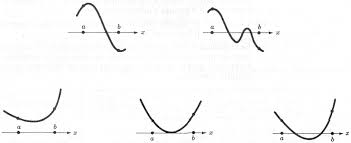
\includegraphics[width=0.8\textwidth]{veeltermen}
  \vfill
\end{center}
% \vfill
\vspace*{-2cm}

\subsection*{Doelstellingen}
{\singlespacing
  Je kan \hfill  {\scriptsize(LP 2005/069, LI 1.2, ET10,11,12,13)}
  \begin{itemize}
  \item vergelijkingen van de eerste en tweede graad in één onbekende oplossen;
  \item veeltermvergelijkingen van graad hoger dan 2 oplossen met behulp van ICT;
  \item aan de hand van het functievoorschrift
    \begin{itemize}
    \item een tabel,
    \item het domein,
    \item de nulwaarden,
    \item het tekenverloop,
    \item de grafiek
    \end{itemize}
    bepalen van veeltermfuncties van de eerste en tweede graad;
  \item aan de hand van de grafiek het stijgen/dalen en de extrema van veeltermfuncties van de eerste en tweede graad bepalen;
  \item met behulp van ICT de tabel en de grafiek lezen(domein, nulwaarden, tekenverloop, stijgen/dalen, extrema) van veeltermfuncties van graad hoger dan twee;
  \item veranderingen bespreken en vergelijken met behulp van differentiequotiënten;
  \item een vraagstuk of probleem, dat aanleiding geeft tot een veeltermfunctie, wiskundig formuleren;
  \item de door het functioneel verband bekomen vergelijking oplossen;
  \item de gevonden oplossing terug vertalen naar de oplossing van het oorspronkelijke vraagstuk of probleem;
  \item problemen met gegeven functioneel verband oplossen en deze oplossing interpreteren.
  \end{itemize}

}
\thispagestyle{empty}
\mbox{}
\newpage
\clearpage
\thispagestyle{empty}
\tableofcontents
\newpage
\clearpage
\pagenumbering{arabic}


\fancyhead[RO,LE]{Veeltermfuncties}
\fancyhead[RE,LO]{}

\onehalfspacing

\section{Veeltermvergelijkingen}

\subsection{Definitie}

\paragraph{Eenterm}
\begin{mdframed}
Een {\bf eenterm} is een product van een coëfficiënt met een macht van een variabele:
$$ax^n\qquad\qquad\mbox{ met }a\in\mathbb{R}, n\in\mathbb{N}$$
\end{mdframed}

\paragraph{Veelterm}
\begin{mdframed}
  Een {\bf reële veelterm} in de variabele $x$ is een som van ééntermen:
  $$ a_nx^n + a_{n-1}x^{n-1} + \cdots + a_1x + a_0 \;.$$
  De reële getallen $a_n, a_{n-1}, \cdots, a_1, a_0$ noemen we de {\bf coëfficiënten} van de veelterm.
  De hoogste exponent bij de variabele $x$ is de {\bf graad} van de veelterm.
\end{mdframed}

\paragraph{Veeltermvergelijking}
\begin{mdframed}
  Een {\bf veeltermvergelijking} in één onbekende $x$ is een vergelijking die in de vorm
  $$a_nx^n + a_{n-1}x^{n-1} + \cdots + a_1x + a_0 = 0$$
  gebracht kan worden.\\
  De hoogste exponent bij de onbekende $x$ is de {\bf graad} van de veelterm.
\end{mdframed}

\begin{oefening}
  Zijn volgende vergelijkingen veeltermvergelijkingen en zo ja, van welke graad?
  \begin{multicols}{2}
    \begin{enumerate}[(a)]
    \item $2x + 2 = 0$
    \item $\sqrt{3x+1} = 0$
    \item $x^2-3x+8=0$
    \item $x^4=-16$
    \end{enumerate}
  \end{multicols}
\end{oefening}

\paragraph{Oplossen van een veeltermvergelijking}
\begin{mdframed}
  Een veeltermvergelijking {\bf oplossen} is het zoeken naar alle onbekenden $x$ zodat de vergelijking waar wordt.
\end{mdframed}

\begin{oefening}
  Beschouw de vergelijking
  $$x^3-6x^2+5x+12=0\;.$$
  \begin{enumerate}[(a)]
  \item Onderzoek of de gehele getallen van -3 tot 3 aan deze vergelijking voldoen.
  \item Zijn er nog andere getallen die aan deze vergelijking voldoen?
  \end{enumerate}
\end{oefening}

\pagebreak
\subsection{Veeltermvergelijkingen van de eerste graad}

\begin{itemize}
\item Synoniem: eerstegraadsvergelijking, lineaire vergelijking
\item Standaardvorm:
  $$ax + b = 0$$
  met $a, b \in \mathbb{R}$ en $a\neq 0$
\item Oplossing:
  $$V=\{-\dfrac{b}{a}\}$$
\end{itemize}

\paragraph{Werkwijze om een eerstegraadsvergelijking op te lossen}
\begin{enumerate}
\item Haakjes wegwerken
\item Noemers wegwerken
\item Onbekenden links, bekenden rechts
\item Vereenvoudigen
\item Onbekende afzonderen
\item Oplossingenverzameling opschrijven en proef maken
\end{enumerate}


\begin{oefening}
  Los de volgende vergelijkingen van de eerste graad op in $\mathbb{R}$
  \begin{multicols}{2}
    \begin{enumerate}[(a)]
      \itemsep0.7em
    \item $4x-8=0$
    \item $3x+9=0$
    \item $-3x+9=0$
    \item $2(x+6)=4-(x+7)$
    \item $x - \dfrac{x-2}{3} = 4$
    \item $2(x-3)+7=5-(2-x)$
    \item $(x+1)^2-2=x(x-3)-(1-2x)$
    \item $\dfrac{3+2x}{4}-\dfrac{4x-5}{5}=\dfrac{21-6x}{6}$
    \item $\dfrac{4x}{3}-\left(\dfrac{3}{2}-\dfrac{x}{4}\right)=x+4\left(\dfrac{2x}{3}-1\right)$
    \item $\dfrac{3(x-1)}{5}-\dfrac{2(1-4x)}{7}=x+\dfrac{x+1}{5}$
    \item $\dfrac{5x}{8}-\dfrac{x-\frac{5}{2}}{4}=1$
    \item $\dfrac{x}{5}+\dfrac{x}{2}=-7$
    \item $\dfrac{3-x}{4}-\dfrac{x-2}{3}=\dfrac{x}{2}-\dfrac{4x+1}{12}$
    \end{enumerate}
  \end{multicols}
\end{oefening}

\pagebreak
\subsection{Veeltermvergelijkingen van de tweede graad}

\begin{itemize}
\item Synoniem: tweedegraadsvergelijking, vierkantsvergelijking, kwadratische vergelijking
\item Standaardvorm:
  $$ax^2 + bx + c = 0$$
  met $a, b, c \in \mathbb{R}$ en $a\neq 0$
\item Volledige tweedegraadsvergelijking:\\
  We noemen een tweedegraadsvergelijking {\bf volledig} als alle coëfficiënten verschillend van nul zijn, d.w.z. als
  $$ a\neq 0 \qquad b\neq 0 \qquad c\neq 0$$
\item Oplossen m.b.v. de discriminantmethode:
  \begin{itemize}
  \item Bereken de discriminant $D=b^2-4ac$
  \item Drie gevallen:
    \begin{itemize}
    \item als $D<0$, dan zijn er geen oplossingen
      $$V=\emptyset$$
    \item als $D>0$, dan zijn er twee verschillende oplossingen: $x_{1,2}=\dfrac{-b\pm\sqrt{D}}{2a}$
      $$V=\{x_1, x_2\}$$
    \item als $D=0$, dan heeft de vergelijking één oplossing (eigenlijk twee samenvallende oplossingen)
      $$V=\{\dfrac{-b}{2a}\}$$
    \end{itemize}
  \end{itemize}
\item Onvolledige tweedegraadsvergelijking:\\
  Een tweedegraadsvergelijking is {\bf onvolledig} als $b=0$ of $c=0$ is. Onvolledige tweedegraadsvergelijkingen kunnen als volgt eenvoudig opgelost worden:
  \begin{itemize}
    \item $b=0$ en $c=0$, dus $ax^2=0$, dan kan $x$ enkel de waarde nul hebben, dus $V=\{0\}$
    \item $b=0$, dus $ax^2+c=0\LRA x^2=\dfrac{-c}{a}$, dus er zijn twee oplossingen als $\dfrac{-c}{a}$ positief is, dus $V=\{-\sqrt{\dfrac{-c}{a}}, +\sqrt{\dfrac{-c}{a}}\}$
    \item $c=0$, dus $ax^2+bx=0\LRA x(ax+b)=0$, dus er zijn altijd twee oplossingen namelijk $x=0$ en de oplossing van de eerstegraadsvergelijking $ax+b=0$, dus $V=\{0, -\dfrac{b}{a}\}$
  \end{itemize}
\end{itemize}


\begin{oefening}
  Los de volgende vergelijkingen van de tweede graad op in $\mathbb{R}$
  \begin{multicols}{2}
    \begin{enumerate}[(a)]
      \itemsep0.7em
    \item $2x^2-4x-6=0$
    \item $5x(x-2)=x(3x-4)-5$
    \item $\frac{2}{3}x^2+5x+1=0$
    \item $80x^2+8x=15$
    \item $80x^2+15=-8x$
    \item $(3-x)(3+x)=(x-4)^2$
    \item $(x-2)^2=x^2-4$
    \item $(3x+2)(3x-2)+6x+5=0$
    \item $x+1=(x+1)(x-1)$
    \item $4x^2-20x+25=0$
    \item $3x^2+5=0$
    \item $x=x^2$
    \item $2\left(7x+32\right)=(3x+8)^2$
    \item $11x+13=2x^2$
    \item $x\left(x+3\right)+2\left(5+2x\right)=0$
    \item $x^2+2x-8=0$
    \item $(x+3)^2=16$
    \item $9x^2+30x+25=0$
    \item $10x^2+7x-3=0$
    \item $x^2=x+1$
    \item $37x^2+13x-50=0$
    \item $3x(3x+10)+5=-20$
    \item $x^2=3x-18$
    \item $x^2=10x-25$
    \end{enumerate}
  \end{multicols}
\end{oefening}

\begin{oefening}
  Los op in $\mathbb{R}$
  \begin{enumerate}[(a)]
      \itemsep1em
    \item $x^2+x-8=(x-6)^2$ \tabto{6cm} {\color{gray}$V=\{\dfrac{44}{13}\}$}
    \item $x^2+\dfrac{15}{2}=\dfrac{11x}{2}$ \tabto{6cm} {\color{gray}$V=\{\dfrac{5}{2}, 3\}$}
    \item $(2x-4)(2x+4)=(x+2)^2$ \tabto{6cm} {\color{gray}$V=\{-2,\dfrac{10}{3}\}$}
    \item $9x^2-36=(6+3x)^2$ \tabto{6cm} {\color{gray}$V=\{-2\}$}
    \item $19-x+x^2=18-2x-x^2$ \tabto{6cm} {\color{gray}$V=\{\}$}
    \item $25x^2+20x=-9$ \tabto{6cm} {\color{gray}$V=\{-\dfrac{3}{5}\}$}
    \item $6x^2=x+1$ \tabto{6cm} {\color{gray}$V=\{-\dfrac{1}{3},\dfrac{1}{2}\}$}
  \end{enumerate}
\end{oefening}

\begin{oefening}
De ring links en de cirkel rechts hebben dezelfde oppervlakte. Bepaal $x$.
\begin{center}
\begin{tikzpicture}[scale=0.6, line cap=round,line join=round,>=triangle 45,x=1.0cm,y=1.0cm]
\clip(-2.05,-0.62) rectangle (18.68,10.69);
\draw [line width=1.2pt,fill=gray!60] (4,5) circle (5cm);
\draw [line width=1.2pt,fill=white] (4,5) circle (3cm);
\draw [line width=1.2pt,fill=gray!60] (14,5) circle (4cm);
\draw [line width=1.2pt] (14,5)-- (16.51,8.12);
\draw [line width=1.2pt] (4,5)-- (5.94,7.29);
\draw [line width=1.2pt,dash pattern=on 2pt off 2pt] (5.94,7.29)-- (7.23,8.82);
\draw (5.8,8.5) node[anchor=north west] {$x$};
\draw (4.3,6.7) node[anchor=north west] {3};
\draw (14.4,6.9) node[anchor=north west] {4};
\fill [color=black] (4,5) circle (1.5pt);
\fill [color=black] (14,5) circle (1.5pt);
\fill [color=black] (7.23,8.82) circle (1.5pt);
\fill [color=black] (16.51,8.12) circle (1.5pt);
\fill [color=black] (5.94,7.29) circle (1.5pt);
\end{tikzpicture}
\end{center}
\end{oefening}

\pagebreak
\subsection{Veeltermvergelijkingen van graad $\geq 3$}

Veeltermvergelijkingen van hogere graad kunnen we oplossen door handmatig (m.b.v. een ZRM) één oplossing $x=a$ te zoeken waardoor we van de veelterm een deler $x-a$ kunnen afsplitsen. De restveelterm kan gevonden worden m.b.v. het {\bf algoritme van Horner}.

\paragraph{Voorbeeld}

We lossen de vergelijking $$x^3-4x^2+x+6=0$$ op.

\begin{itemize}
\item Zoek een $x$ zodat de vergelijking waar wordt:
  \begin{description}
  \item[$x=1$] $\rightarrow 1^3-4\cdot 1^2+1+6 = 4 \neq 0$
  \item[$x=0$] $\rightarrow 0^3-4\cdot 0^2+0+6 = 6 \neq 0$
  \item[$x=-1$] $\rightarrow (-1)^3-4\cdot (-1)^2+(-1)+6 = 0$
  \end{description}
\item Dus $x=-1$ is een oplossing. Dit wil zeggen dat $x-(-1)$ of korter $x+1$ een deler is van de de veelterm. We herschrijven de vergelijking:
  \begin{eqnarray*}
    x^3-4x^2+x+6&=&0\\
    \LRA (x+1)\underbrace{(\qquad ? \qquad)}_{\mbox{restveelterm}}&=&0\\
  \end{eqnarray*}
\item De restveelterm vinden we m.b.v. het algoritme van Horner:
  \begin{center}
    \begin{tabular}{c|cccc}
      & 1 & -4 & 1 & 6\\
      -1 & $\downarrow$ & -1 & 5 & -6\\
      \hline
      & 1 & -5 & 6 & 0
    \end{tabular}
  \end{center}
\item We krijgen dus:
  \begin{eqnarray*}
    x^3-4x^2+x+6&=&0\\
    \LRA (x+1)(x^2-5x+6)&=&0\\
  \end{eqnarray*}
\item Voor de factor $(x+1)$ hebben we reeds de oplossing $x_0=-1$ gevonden. Ook de factor $(x^2-5x+6)$ heeft oplossingen. Deze vinden we m.b.v. de discriminantmethode:
  $$x^2-5x+6=0$$
  $$D=25-4\cdot 1\cdot 6=1$$
  $$x_{1,2}=\dfrac{5\pm 1}{2}=3\mbox{ en }2$$
\item Dus $x^3-4x^2+x+6=0$ heeft als oplossingenverzameling
  $$V=\{-1, 2, 3\}$$
\end{itemize}

\begin{oefening}
  Los op in $\mathbb{R}$
  \begin{multicols}{2}
    \begin{enumerate}[(a)]
    \itemsep0.7em
    \item $x^3+2x-3=0$
    \item $7x^3+8x^2+3x+2=0$
    \item $x^3-x+6=0$
    \item $3x^2(x-1)=\dfrac{7}{2}x^2-2$
    \item $8x^3+12x^2+6x+2=0$
    \item $20x^3+60x^2+45x=0$
    \item $x^4-4x^3-x^2+16x-12=0$
    \item $x+\dfrac{7x}{2}=\dfrac{3x^3}{2}+\dfrac{3x^2}{2}+\dfrac{3}{2}$
    \item $x^3+(2x+1)^2=x+1$
    \end{enumerate}
  \end{multicols}
\end{oefening}

\begin{oefening} % www3.ul.ie/~mlc/support/.../chap3/3_3.pdf
  Los volgende vergelijkingen van graad hoger dan twee op in $\mathbb{R}$:
  %\begin{multicols}{2}
  \begin{enumerate}[(a)]
  \itemsep.7em
  \item $x^3-17x^2+54x-8=0$
  \item $x^3-6x^2+11x-6=0$
  \item $x^3-7x=6$
  \item $2x^3+9x^2+7x+2=2x^2$
  \item $22x+8=3x^3+7x^2$
  \item $2x^4+8x^3-\dfrac{7x^2}{2}-\dfrac{67x}{2}-15=0$
  \item $4x^4+8x^3+3x^2-2x-1=0$
  \end{enumerate}
  %\end{multicols}
\end{oefening}

\pagebreak

\subsection{Veeltermvergelijkingen oplossen m.b.v. Geogebra}

\subsection*{Eerste methode}

\paragraph*{Voorbeeld:} Los op in $\mathbb{R}$
$$x^3-2x^2-1=x^2+x-4$$

Beschouw het linkerlid en het rechterlid als functies:
$$f(x)=x^3-2x^3-1$$
$$g(x)=x^2+x-4$$

Voor alle $x$ die een oplossing zijn van de originele vergelijk geldt dus dat
$$f(x)=g(x)$$

Construeer nu de grafieken van $f(x)$ en van $g(x)$ met Geogebra. Download het programma op \url{https://www.geogebra.org/} als dit nog niet geïnstalleerd is. Hiervoor moet je onderaan in het commandovenster het commando \verb#f(x)=x^3-2*x^3-1# en \verb#g(x)=x^2+x-4# invoeren.

Voor de snijpunten van de grafieken geldt nu dus dat $f(x)=g(x)$. En we zoeken de $x$-waarden om de originele vergelijking waar te maken. In het menu van Geogebra moeten we dus op zoek naar het icoon om het snijpunt van de twee grafieken te bepalen. Eenmaal dat we alle snijpunten hebben moeten we maar enkel de verschillende $x$-waarden van deze punten aflezen om de oplossingenverzameling te bepalen:

$$V=\{-1, 1, 3\}$$

\subsection*{Tweede methode}

\paragraph*{Voorbeeld:} Los op in $\mathbb{R}$
$$x^3-2x^2-1=x^2+x-4$$

We herschrijven deze vergelijking eerst in zijn standaardvorm:
$$\LRA x^3-3x^2-x + 3=0$$

We hoeven nu enkel het linkerlid als de functie
$$f(x)=x^3-3x^2-x + 3$$
te plotten. Want als we naar de vergelijking in standaardvorm kijken zoeken we eigenlijk de nulwaarden van deze functie.

Construeer de grafiek van deze functie $f$ in Geogebra en lees de nulwaarde af via het menu snijpunten van 2 objecten. Je zou dezelfde oplossingenverzameling

$$V=\{-1, 1, 3\}$$

moeten vinden.

\begin{oefening}
  Los op in $\mathbb{R}$\\
  \begin{enumerate}[(a)]
    \itemsep2em
  \item $\displaystyle\frac{{x}^{6}}{2}+\frac{21\,{x}^{5}}{4}+\frac{81\,{x}^{4}}{4}+\frac{67\,{x}^{3}}{2}+18\,{x}^{2}=\frac{27\,x}{4}+\frac{27}{4}$
  \item $\displaystyle{x}^{3}+\frac{7\,{x}^{2}}{2}+x=\frac{3}{2}$
  \end{enumerate}
\end{oefening}

\begin{oefening}
  Los volgende vergelijkingen op in $\mathbb{R}$ door gebruik te maken van Horner, controleer daarna je antwoord m.b.v. ICT.\\
  \begin{enumerate}[(a)]
    \itemsep1em
  \item $\displaystyle{x}^{3}+{x}^{2}=2\,x$
  \item $\displaystyle{x}^{6}-{x}^{5}-13\,{x}^{4}=-13\,{x}^{3}-36\,{x}^{2}+36\,x$
  \end{enumerate}
\end{oefening}

\begin{oefening}
  Maak gebruik van Geogebra om de volgende vergelijkingen op te lossen in $\mathbb{R}$
  \begin{multicols}{2}
    \begin{enumerate}[(a)]
      \itemsep0.7em
    \item $-5x+4=0$
    \item $2(x+6)=4-(x+7)$
    \item $2x^2-4x-6=0$
    \item $5x(x-2)=x(3x-4)-5$
    \item $3x^3+x^2-8x+4=0$
    \item $x^3+6x^2-x-30=0$
    \item $x^3-3x^2+4=0$
    \item $-4(x-5)=3(2x+1)$
    \item $(x+\sqrt{5})(x^2+2x-8)=0$
    \item $5x^2+3x-4=0$
    \end{enumerate}
  \end{multicols}
\end{oefening}


\newpage

\section{Veeltermfuncties}

\subsection{Definities}

\paragraph*{Veeltermfunctie}
\begin{mdframed}
  Een {\bf veeltermfunctie} is een reële functie waarvan het functievoorschrift gegeven wordt door een veelterm:
  $$f(x)= a_nx^n + a_{n-1}x^{n-1} + \cdots + a_1x + a_0$$
\end{mdframed}

De {\bf graad van de veeltermfunctie} is gelijk aan de graad van de veelterm. In de definitie is de veeltermfunctie dus van de $n$-de graad.

\begin{oefening}
  Welke van de volgende functies zijn veeltermfuncties. Als het veeltermfuncties zijn, wat is dan hun graad?
\begin{multicols}{2}
  \begin{enumerate}[(a)]
  \itemsep1em
  \item $f(x)=\dfrac{2}{3}x+2$
  \item $f(x)=0.5x^2-x-1.5$
  \item $f(x)=\sqrt{3x^2+2x-6}$
  \item $f(x)=-\dfrac{3}{4}x^2+3x$
  \item $f(x)=\dfrac{3}{x^2}+\dfrac{2}{x}+1$
  \item $f(x)=42$
  \item $f(x)=3x^2-0.5x^3$
  \item $f(x)=2^x+2$
  \end{enumerate}
\end{multicols}
\end{oefening}

\begin{oefening}
Schrijf volgende veeltermfuncties in hun standaardvorm.
\begin{multicols}{2}
  \begin{enumerate}[(a)]
  \itemsep1em
  \item $f(x)=2+x^3-x^2$
  \item $f(x)=-(x^2-2x+3)$
  \item $f(x)=3x(x^2-2x+3)$
  \item $f(x)=(x-2)(x+3)$
  \item $f(x)=(x-2)^2$
  \item $f(x)=(2x-3)^2$
  \item $f(x)=(x^2+2x)^2$
  \item $f(x)=(2x-4)^3$
  \item $f(x)=\dfrac{1}{7}(x-2)^2$
  \item $f(x)=\dfrac{x+2}{3}\cdot\dfrac{x-2}{2}$
  \end{enumerate}
\end{multicols}
\end{oefening}

\pagebreak
\subsection{Veeltermfuncties van graad 0}

\begin{itemize}
\item Synoniemen voor deze functies zijn nulveeltermfuncties of {\bf constante functies}. Wij zullen vanaf nu de benaming constante functie gebruiken.
\item Deze functies hebben de vorm
  $$f(x) = a$$
  met $a$ een reëel getal.
\item De grafiek van deze functie is een horizontale rechte evenwijdig met de $x$-as.
\item Het domein is dus $\mathbb{R}$
\item De grafiek van deze functie snijdt de $y$-as in het punt $(0, a)$.
\item Als $a\neq 0$ dan heeft deze functie geen nulwaarden.
\item Als $a=0$ dan heeft deze functie alle reële getallen als nulwaarden.
\end{itemize}

\begin{oefening}
  Beschouw de functie
  $$f(x)=-2\;.$$
  \begin{enumerate}[(a)]
  \item Dit is een veeltermfunctie van de hoeveelste graad?
  \item Hoe noemen we zulk een functie?
  \item Hoe ziet deze functie eruit?
  \item Wat zijn de nulwaarden?
  \item Teken de grafiek zonder een functiewaardentabel te maken.
  \end{enumerate}
\end{oefening}

\paragraph*{Constante functie bespreken}
\begin{mdframed}
  \begin{itemize}
  \item Functievoorschrift: $f(x)=a$
  \item $\dom f = \mathbb{R}$ en $\ber f = \{a\}$
  \item Nulwaarden:
    \begin{itemize}
    \item Als $a\neq 0$ dan geen nulwaarden.
    \item Als $a=0$ dan zijn de nulwaarden $\mathbb{R}$.
    \end{itemize}
  \item Tekenverloop:
    \begin{center}
      \begin{tabular}{c|lcr}
        $x$ & $-\infty$ & & $+\infty$\\
        \hline
        $f(x)$ & & teken van $a$ &
      \end{tabular}
    \end{center}
  \item Functiewaardentabel en grafiek: /
  \end{itemize}
\end{mdframed}

\begin{oefening}
  Beschrijf volgende constante functies:
  \begin{enumerate}[(a)]
  \item $f(x)=42$
  \item $f(x)=0$
  \end{enumerate}
\end{oefening}

\begin{oefening}
  Geef het functievoorschrift van de rechte die door de punten $(-2,1.5)$ en $(3,1.5)$ gaat.
\end{oefening}

\begin{oefening}
  Geef het functievoorschrift van de volgende grafiek:
  \begin{center}
    \definecolor{cqcqcq}{rgb}{0.75,0.75,0.75}
    \begin{tikzpicture}[line cap=round,line join=round,>=triangle 45,x=1.0cm,y=1.0cm]
      \draw [color=cqcqcq,dash pattern=on 1pt off 1pt, xstep=2.0cm,ystep=2.0cm] (-4.62,-4.36) grid (8.32,4.42);
      \draw[->,color=black] (-4.62,0) -- (8.32,0);
      \foreach \x in {-4,-2,2,4,6,8}
      \draw[shift={(\x,0)},color=black] (0pt,2pt) -- (0pt,-2pt) node[below] {\footnotesize $\x$};
      \draw[->,color=black] (0,-4.36) -- (0,4.42);
      \foreach \y in {-4,-2,2,4}
      \draw[shift={(0,\y)},color=black] (2pt,0pt) -- (-2pt,0pt) node[left] {\footnotesize $\y$};
      \draw[color=black] (0pt,-10pt) node[right] {\footnotesize $0$};
      \clip(-4.62,-4.36) rectangle (8.32,4.42);
      \draw[line width=2pt, smooth,samples=100,domain=-4.620000000000001:8.320000000000006] plot(\x,{0-3});
      \draw (4.74,-2.35) node[anchor=north west] {$f(x)$};
    \end{tikzpicture}
  \end{center}
\end{oefening}

\pagebreak
\subsection{Veeltermfuncties van graad 1}

\begin{itemize}
\item Synoniemen voor deze functies zijn {\bf eerstegraadsfuncties} of lineaire functies. Wij zullen vanaf nu de benaming eerstegraadsfunctie gebruiken.
\item Deze functies hebben de vorm
  $$f(x) = ax+b $$
  met $a$ en $b$ een reëel getallen en $a$ verschillend van $0$.
\item De grafiek van deze functie is een schuine rechte die stijgt indien $a > 0$ en daalt indien $a<0$.
\item De coëfficiënt $a$ wordt de richtingscoëfficiënt genoemd, het is een maat voor de helling van de rechte ten opzichte van de $x$-as.
\item Het domein is dus $\mathbb{R}$.
\item De grafiek van deze functie snijdt de $x$-as in het punt $(-\dfrac{b}{a}, 0)$ en $x_0=-\dfrac{b}{a}$ is de enige nulwaarde van de functie.
\item De grafiek van deze functie snijdt de $y$-as in het punt $(0, b)$. De constante term $b$ bepaalt dus waar de grafiek de $y$-as snijdt.
\item De grafiek van deze functie heeft geen extrema.
\end{itemize}

\begin{oefening}
  Beschouw de functie
  $$f(x)=-\dfrac{1}{2}x+2\;.$$
  \begin{enumerate}[(a)]
  \item Dit is een veeltermfunctie van de hoeveelste graad?
  \item Hoe noemen we zulk een functie?
  \item Hoe ziet deze functie eruit?
  \item Wat zijn de nulwaarden?
  \item Waar snijdt deze functie de assen?
  \item Teken de grafiek zonder een functiewaardentabel te maken.
  \end{enumerate}
\end{oefening}

\paragraph*{Eerstegraadsfunctie bespreken}
\begin{mdframed}
  \begin{itemize}
  \item Functievoorschrift: $f(x)=ax + b$
  \item $\dom f = \mathbb{R}$ en $\ber f = \mathbb{R}$
  \item Nulwaarde: $x_0=-\dfrac{b}{a}$
  \item Tekenverloop:
    \begin{center}
      \begin{tabular}{c|lp{2.5cm}cp{1.5cm}r}
        $x$ & $-\infty$ & & $x_0$ & & $+\infty$\\
        \hline
        $f(x)$ & & tegengesteld teken van $a$ & 0 & teken van $a$ &
      \end{tabular}
    \end{center}
  \item Functiewaardentabel: twee, hoogstens drie koppels is voldoende
  \item Grafiek maken
  \item Stijgen\&dalen:\\
    \begin{minipage}{0.45\textwidth}
      \centering $a>0$\\
      \begin{tabular}{c|lcr}
        $x$ & $-\infty$ & & $+\infty$\\
        \hline
        $f(x)$ & & $\nearrow$ &
      \end{tabular}
    \end{minipage}
    \begin{minipage}{0.45\textwidth}
      \centering $a<0$\\
      \begin{tabular}{c|lcr}
        $x$ & $-\infty$ & & $+\infty$\\
        \hline
        $f(x)$ & & $\searrow$ &
      \end{tabular}
    \end{minipage}
  \end{itemize}
\end{mdframed}

\begin{oefening}
  Beschrijf volgende eerstegraadsfuncties:
  \begin{enumerate}[(a)]
  \item $f(x)=2x-3$
  \item $f(x)=-x+4$
  \end{enumerate}
\end{oefening}

\begin{oefening}
  Bepaal het functievoorschrift van
  \begin{enumerate}[(a)]
  \item de rechte door $(-2, 3)$ en $(1, 0)$.
  \item de rechte door $(-2, 0)$ en $(1, 3)$.
  \item de rechte door $(1, -1)$ en $(3, -1)$.
  \item de rechte door $(3, -1)$ en $(3, 6)$.
  \end{enumerate}
\end{oefening}

\begin{oefening}
  Teken de grafiek van de eerstegraadsfunctie die als nulwaarde $x=3$ heeft en die de $y$-as snijdt in het punt $(0,-6)$. Kan je het functievoorschrift vinden voor deze functie?
\end{oefening}

\begin{oefening}
  Geef het functievoorschrift van de volgende grafiek:
  \begin{center}
    \definecolor{cqcqcq}{rgb}{0.75,0.75,0.75}
    \begin{tikzpicture}[scale=0.75, line cap=round,line join=round,>=triangle 45,x=1.0cm,y=1.0cm]
      \draw [color=cqcqcq,dash pattern=on 1pt off 1pt, xstep=2.0cm,ystep=2.0cm] (-4.54,-2.74) grid (8.56,4.62);
      \draw[->,color=black] (-4.54,0) -- (8.56,0);
      \foreach \x in {-4,-2,2,4,6,8}
      \draw[shift={(\x,0)},color=black] (0pt,2pt) -- (0pt,-2pt) node[below] {\footnotesize $\x$};
      \draw[->,color=black] (0,-2.74) -- (0,4.62);
      \foreach \y in {-2,2,4}
      \draw[shift={(0,\y)},color=black] (2pt,0pt) -- (-2pt,0pt) node[left] {\footnotesize $\y$};
      \draw[color=black] (0pt,-10pt) node[right] {\footnotesize $0$};
      \clip(-4.54,-2.74) rectangle (8.56,4.62);
      \draw[line width=2pt, smooth,samples=100,domain=-4.540000000000001:8.560000000000006] plot(\x,{0-0.5*(\x)+3});
      \draw (0.68,3.22) node[anchor=north west] {$f$};
    \end{tikzpicture}
  \end{center}
\end{oefening}


\pagebreak
\subsection{Veeltermfuncties van graad 2}

\begin{itemize}
\item Synoniemen voor deze functies zijn {\bf tweedegraadsfuncties} of kwadratische functies. Wij zullen vanaf nu de benaming tweedegraadsfunctie gebruiken.
\item Deze functies hebben de vorm
  $$f(x) = ax^2+bx+c $$
  met $a$, $b$ en $c$ een reëel getallen en $a$ verschillend van $0$.
\item We kunnen voor elke reële waarde de functiewaarde bereken, dus het domein is $\mathbb{R}$.
\item De grafiek van deze functie is een parabool met symmetrieas evenwijdig met de $y$-as.
\item Als $a>0$ dan opent de parabool zich naar boven en dat noemen we een {\bf dalparabool}.
\item Als $a<0$ dan opent de parabool zich naar beneden en dat noemen we een {\bf bergparabool}.
\item De top van de parabool bevindt zich in het punt $(-\dfrac{b}{2a}, f(-\dfrac{b}{2a}))$. Dit punt kan ook berekend worden met $(-\dfrac{b}{2a}, -\dfrac{D}{4a})$, waarbij we $D=b^2-4ac$ de discriminant noemen.
\item De top is het extrema van de functie, een maximum als $a<0$ en een minimum als $a>0$.
\item Een tweedegraadsfunctie kan $0, 1$ of $2$ nulwaarden hebben, afhankelijk van de discriminant.
\end{itemize}

\begin{oefening}
  Beschouw de functie
  $$f(x)=x^2-x-6\;.$$
  \begin{enumerate}[(a)]
  \item Dit is een veeltermfunctie van de hoeveelste graad?
  \item Hoe noemen we zulk een functie?
  \item Hoe ziet deze functie eruit?
  \item Wat zijn de nulwaarden?
  \item Waar snijdt deze functie de assen?
  \item Heeft deze functie een extremum, waar ligt dit extremum en hoe noemen we dit extremum in deze context?
  \item Teken de grafiek zonder een functiewaardentabel te maken.
  \end{enumerate}
\end{oefening}

\pagebreak
\paragraph*{Tweedegraadsfuncties bespreken}
\begin{mdframed}
  \begin{itemize}
  \item Functievoorschrift: $f(x)=ax^2 + bx + c$
  \item $a>0$ dan een dalparabool, $a<0$ dan een bergparabool
  \item $\dom f = \mathbb{R}$
  \item $a>0$ dan $\ber f = [f(-\dfrac{b}{2a}), +\infty]$, $a<0$ dan $\ber f = [-\infty, f(-\dfrac{b}{2a})]$
  \item Nulwaarden: $ax^2+bx+c=0$
    \renewcommand{\labelitemii}{$\bullet$}
    \begin{itemize}
    \item $D=b^2-4ac$
    \item $D>0$ dan twee verschillende nulwaarden $x_1=\dfrac{-b-\sqrt{D}}{2a}$ en $x_0=\dfrac{-b+\sqrt{D}}{2a}$
    \item $D=0$ dan één nulwaarde $x_0=-\dfrac{b}{2a}$
    \item $D<0$ dan geen nulwaarden
    \end{itemize}
  \item Tekenverloop:
    \begin{itemize}
    \item $D>0$
      \begin{tabular}{c|p{1.5cm}cp{2.5cm}cp{1.5cm}}
        $x$ & & $x_1$ & & $x_2$ &\\
        \hline
        $f(x)$ & teken van $a$ & 0 & tegengesteld teken van $a$ & 0 & teken van $a$
      \end{tabular}
    \item $D=0$
      \begin{tabular}{c|lp{1.5cm}cp{1.5cm}r}
        $x$ & $-\infty$ & & $x_0$ & & $+\infty$\\
        \hline
        $f(x)$ & & teken van $a$ & 0 & teken van $a$ &
      \end{tabular}
    \item $D<0$
      \begin{tabular}{c|lcr}
        $x$ & $-\infty$ &  & $+\infty$\\
        \hline
        $f(x)$ & & teken van $a$ &
      \end{tabular}
    \end{itemize}
  \item Functiewaardentabel: kies de nulwaarden en nog een aantal $x$-waarden daarrond
  \item Grafiek maken
  \item Stijgen\&dalen:\\
    \begin{minipage}{0.45\textwidth}
      \centering $a>0$\\
      \begin{tabular}{c|lcr}
        $x$ &  & $-\dfrac{b}{2a}$ & \\[0.1cm]
        \hline
        $f(x)$ & $\searrow$ & $\underset{=f(-\frac{b}{2a})}{\mbox{min}}$ & $\nearrow$
      \end{tabular}
    \end{minipage}
    \begin{minipage}{0.45\textwidth}
      \centering $a<0$\\
      \begin{tabular}{c|lcr}
        $x$ &  & $-\dfrac{b}{2a}$ & \\[0.1cm]
        \hline
        $f(x)$ & $\nearrow$ & $\underset{=f(-\frac{b}{2a})}{\mbox{max}}$ & $\searrow$
      \end{tabular}
    \end{minipage}
  \end{itemize}
\end{mdframed}

\begin{oefening}
  Bespreek de volgende functies:
  \begin{multicols}{2}
  \begin{enumerate}[(a)]
  \item $f(x)=x^2+x-6$
  \item $f(x)=x^2+2x+1$
  \item $f(x)=x^2+4$
  \item $f(x)=3x-2$
  \item $f(x)=-2x^2-3x+1$
  \item $f(x)=4x^2-4x-15$

  \item $f(x)=(x+2)^2-4$
  \item $f(x)=4x+(x-2)^2$
  \item $f(x)=(x-2)(x+2)$
  \item $f(x)=(x+3)^2+(x-3)^2$
  \item $f(x)=-(x-1)(x+1)$
  \item $f(x)=-2x^2+29x-102$
  \end{enumerate}
  \end{multicols}
\end{oefening}

\begin{oefening}
  Zoek het functievoorschrift van de functie $f$ die door de punten $(-1,0)$, $(0,3)$, $(1,4)$ en $(3,0)$ gaat, zie onderstaande grafiek.
  \begin{center}
    \definecolor{cqcqcq}{rgb}{0.75,0.75,0.75}
    \begin{tikzpicture}[scale=0.9, line cap=round,line join=round,>=triangle 45,x=1.0cm,y=1.0cm]
      \draw [color=cqcqcq,dash pattern=on 1pt off 1pt, xstep=1.0cm,ystep=1.0cm] (-2.55,-2.69) grid (5.45,5.36);
      \draw[->,color=black] (-2.55,0) -- (5.45,0);
      \foreach \x in {-2,-1,1,2,3,4,5}
      \draw[shift={(\x,0)},color=black] (0pt,2pt) -- (0pt,-2pt) node[below] {\footnotesize $\x$};
      \draw[->,color=black] (0,-2.69) -- (0,5.36);
      \foreach \y in {-2,-1,1,2,3,4,5}
      \draw[shift={(0,\y)},color=black] (2pt,0pt) -- (-2pt,0pt) node[left] {\footnotesize $\y$};
      \draw[color=black] (0pt,-10pt) node[right] {\footnotesize $0$};
      \clip(-2.55,-2.69) rectangle (5.45,5.36);
      \draw[line width=2pt, smooth,samples=100,domain=-2.545454545454543:5.4545454545454595] plot(\x,{0-(\x)^2+2*(\x)+3});
      \draw (2.45,2.89) node[anchor=north west] {$f$};
      \begin{scriptsize}
        \fill [color=black] (1,4) circle (2.0pt);
        \draw[color=black] (1.29,4.4) node {$(1, 4)$};
        \fill [color=black] (0,3) circle (2.0pt);
        \draw[color=black] (0.45,2.96) node {$(0, 3)$};
        \fill [color=black] (-1,0) circle (2.0pt);
        \draw[color=black] (-1.42,0.42) node {$(-1, 0)$};
        \fill [color=black] (3,0) circle (2.0pt);
        \draw[color=black] (3.38,0.42) node {$(3, 0)$};
      \end{scriptsize}
    \end{tikzpicture}
  \end{center}
\end{oefening}


\begin{oefening}
  Teken de grafiek van de tweedegraadsfunctie die de nulwaarden $x_1=-2$ en $x_2=1$ heeft en die als top het punt $(-0.5,-2.25)$ heeft. Je weet verder nog dat de grafiek de $y$-as snijdt in het punt $(0,-2)$. Kan je het functievoorschrift vinden voor deze functie?
\end{oefening}

\begin{oefening}
Een landbouwer beschikt over $800 \m$ prikkeldraad. Hij wil daarmee een zo groot mogelijk rechthoekig stuk land afspannen. Aan één zijde is geen prikkeldraad nodig want daar loopt een rivier.
\begin{enumerate}[(a)]
  \item Maak een schets van het probleem. Noem de lengte van het stuk land $l$ en de breedte $b$.
  \item Welk verband is er tussen de lengte $l$, de breedte $b$ en het getal $800$?
  \item Welke formule gebruik je om de oppervlakte van het stuk land te berekenen?
  \item Neem $l$ of $b$ als onbekende $x$ en druk de andere uit in functie van $x$.
  \item Voor het oppervlakte krijg je nu een functie $f$ met maar één onbekende $x$. Bepaal daar het maximum van.
  \item Welke lengte en breedte moet de landbouwer dus kiezen?
\end{enumerate}
\end{oefening}


\pagebreak
\subsection{Veeltermfuncties van graad 3 of hoger}

\begin{itemize}
\item We noemen zulk een functie wel nog eens een {\bf hogeregraadsveeltermfunctie}.
\item Deze functies hebben de algemene vorm van een veeltermfunctie
  $$f(x)= a_nx^n + a_{n-1}x^{n-1} + \cdots + a_1x + a_0\;.$$
\item We kunnen voor elke reële waarde de functiewaarde bereken, dus het domein is $\mathbb{R}$.
\item Een veeltermfunctie van graad $n$ heeft hoogstens $n$ nulwaarden.
\item Veelal vinden we de nulwaarden m.b.v. Horner.
\end{itemize}

\paragraph*{Hogeregraadsveeltermfuncties bespreken}
\begin{mdframed}
  \begin{itemize}
  \item Functievoorschrift: $f(x)= a_nx^n + a_{n-1}x^{n-1} + \cdots + a_1x + a_0\;.$
  \item $\dom f = \mathbb{R}$
  \item Nulwaarden bepalen, bijvoorbeeld m.b.v. Horner.
  \item Functiewaardentabel maken, zorg dat de nulwaarden en voldoende waarden rond de nulwaarde in de tabel staan.
  \item Grafiek maken.
  \item Bereik: a.d.h.v. de grafiek
  \item Tekenverloop: a.d.h.v. de grafiek
  \item Stijgen\&dalen: a.d.h.v. de grafiek
  \end{itemize}
\end{mdframed}

\begin{oefening}
  Bespreek volgende functies:
  \begin{enumerate}[(a)]
  \itemsep.5em
  \item $f(x)=\dfrac{1}{10}(-2x^3-11x^2+21x+90)$
  \item $f(x)=3x^2-0.5x^3$
  \item $f(x)=2x^4+7x^3-51x^2-7x+49$
  \item $f(x)=-21x^4-143x^3+197x^2-25x-8$£
  \item $f(x)=x^5-5x^3+4x$
  \item $f(x)=x^3+3x^2-x-3$
  \item $f(x)=x^4-x^3-10.25x^2+5.25x+22.5$
  \end{enumerate}
\end{oefening}

\pagebreak
\subsection{Hogeregraadsveeltermfuncties bespreken met behulp van Geogebra}
Alternatief kunnen we ook I.C.T., zoals bijvoorbeeld het programma {\em Geogebra} gebruiken om hogeregraadsveeltermfuncties te bespreken. We plotten eerst de grafiek en bespreken daarna alle karakteristieken.

\begin{oefening}
  Met Geogebra werd de grafiek van de functie met functievoorschrift
  $$f(x)=x^5-5x^3+4x$$ gegenereerd. Lees aan de hand van de grafiek het domein, de nulwaarden en de extrema af. Bepaal het tekenverloop, het stijgen en dalen en de symmetrieën van de functie.
  \begin{center}
    \definecolor{cqcqcq}{rgb}{0.75,0.75,0.75}
    \begin{tikzpicture}[scale=0.7, line cap=round,line join=round,>=triangle 45,x=1.0cm,y=1.0cm]
      \draw [color=cqcqcq,dash pattern=on 2pt off 2pt, xstep=1.0cm,ystep=1.0cm] (-7.22,-6.82) grid (8.13,6.66);
      \draw[->,color=black] (-7.22,0) -- (8.13,0);
      \foreach \x in {-7,-6,-5,-4,-3,-2,-1,1,2,3,4,5,6,7,8}
      \draw[shift={(\x,0)},color=black] (0pt,2pt) -- (0pt,-2pt) node[below] {\footnotesize $\x$};
      \draw[color=black] (7.87,0.07) node [anchor=south west] { x};
      \draw[->,color=black] (0,-6.82) -- (0,6.66);
      \foreach \y in {-6,-5,-4,-3,-2,-1,1,2,3,4,5,6}
      \draw[shift={(0,\y)},color=black] (2pt,0pt) -- (-2pt,0pt) node[left] {\footnotesize $\y$};
      \draw[color=black] (0.08,6.33) node [anchor=west] { y};
      \draw[color=black] (0pt,-10pt) node[right] {\footnotesize $0$};
      \clip(-7.22,-6.82) rectangle (8.13,6.66);
      \draw[line width=1.6pt, smooth,samples=100,domain=-2.2:2.2] plot(\x,{(\x)^5-5*(\x)^3+4*(\x)});
    \end{tikzpicture}
  \end{center}
\end{oefening}

\newpage
\section{Differentiequotiënt}

\subsection{Voorbeeld}

Een hardloper houdt tijdens een training van een half uur zijn tussentijden bij:

\hspace*{2cm}
\begin{tabular}{r|cccc}
  tijd $t$ (in minuten) & 0 & 10 & 15 & 30\\
  \hline
  afstand $s$ (in kilometer) & 0 & 3.5 & 5.5 & 8
\end{tabular}

Als hij terug thuis is vraagt hij zich af in welk tijdsinterval hij het snelst liep. Hij maakt de volgende grafiek:\\

\begin{center}
  \begin{tikzpicture}[xscale=1, line cap=round,line join=round,>=triangle 45,x=0.5cm,y=0.8cm]
    \draw[->,color=black] (-1.53,0) -- (32.33,0);
    \foreach \x in {,2,4,6,8,10,12,14,16,18,20,22,24,26,28,30}
    \draw[shift={(\x,0)},color=black] (0pt,2pt) -- (0pt,-2pt) node[below] {\footnotesize $\x$};
    \draw[->,color=black] (0,-0.44) -- (0,8.5);
    \foreach \y in {,1,2,3,4,5,6,7}
    \draw[shift={(0,\y)},color=black] (2pt,0pt) -- (-2pt,0pt) node[left] {\footnotesize $\y$};
    \draw[color=black] (0pt,-10pt) node[right] {\footnotesize $0$};
    \clip(-1.53,-1) rectangle (32.33,8.5);
    \draw [line width=1.6pt] (0,0)-- (10,3.5);
    \draw [line width=1.6pt] (10,3.5)-- (15,5.5);
    \draw [line width=1.6pt] (15,5.5)-- (30,8);
    \begin{scriptsize}
      \fill [color=black] (0,0) circle (2.5pt);
      \draw[color=black] (1.95,0.25) node {$(0, 0)$};
      \fill [color=black] (10,3.5) circle (2.5pt);
      \draw[color=black] (8.48,3.66) node {$(10, 3.5)$};
      \fill [color=black] (15,5.5) circle (2.5pt);
      \draw[color=black] (16.59,5.4) node {$(15, 5.5)$};
      \fill [color=black] (30,8) circle (2.5pt);
      \draw[color=black] (28.8,8.2) node {$(30, 8)$};
    \end{scriptsize}
    \draw[color=black] (32,-0.4) node {$t$};
    \draw[color=black] (-0.8,8.2) node {$s$};
  \end{tikzpicture}
\end{center}

Het is aan de grafiek duidelijk dat de loper niet langer hard liep in het laatste interval $[15, 30]$. Maar hoe zit het in de intervallen $[0,10]$ en $[10,15]$. We delen hiervoor de afgelegde afstand door de tijd. We krijgen met andere woorden de snelheid in $\kmpermin$ of omgevormd in $\kmperh$.

\begin{itemize}
\item Op het tijdsinterval $[0, 10]$ berekenen we
  $$\dfrac{3.5-0}{10-0}=\dfrac{3.5}{10}=0.35$$
  De gemiddelde snelheid in dat interval is dus $0.35 \kmpermin = 21 \kmperh$
\item Op het tijdsinterval $[10, 15]$ berekenen we
  $$\dfrac{5.5-3.5}{15-10}=\dfrac{2}{5}=0.4$$
  De gemiddelde snelheid in dat interval is dus $0.4 \kmpermin = 24 \kmperh$
\item Op het tijdsinterval $[15, 20]$ berekenen we
  $$\dfrac{8-5.5}{30-15}=\dfrac{2.5}{15}=0.1666\ldots$$
  De gemiddelde snelheid in dat interval is dus $0.1666\ldots \kmpermin = 10 \kmperh$
\end{itemize}

Dus door de afgelegde afstand te delen door de lengte van het tijdsinterval vinden we de gemiddelde snelheid. Eigenlijk berekenen we zo de gemiddelde verandering over dat interval. Dit wordt het differentiequotiënt in dat interval genoemd.

\subsection{Definitie}

\paragraph{Differentiequotiënt}
\begin{mdframed}
  het differentiequotiënt $\dfrac{\Delta y}{\Delta x}$ van een functie $f$ voor een interval $[a, b]$ is de gemiddelde verandering van deze functie in interval. We bereken
  $$\dfrac{\Delta y}{\Delta x}=\dfrac{f(b)-f(a)}{b-a}$$
\end{mdframed}


\begin{center}
  \begin{tikzpicture}[scale=2, line cap=round,line join=round,>=triangle 45,x=1.0cm,y=1.0cm]
    \draw[->,color=black] (-0.5,0) -- (3.33,0);
    \foreach \x in {-0.5,0.5,1,1.5,2,2.5,3}
    \draw[shift={(\x,0)},color=black] (0pt,2pt) -- (0pt,-2pt);
    \draw[->,color=black] (0,-0.65) -- (0,3.13);
    \foreach \y in {-0.5,0.5,1,1.5,2,2.5,3}
    \draw[shift={(0,\y)},color=black] (2pt,0pt) -- (-2pt,0pt);
    \clip(-0.5,-0.65) rectangle (3.33,3.13);
    \draw[line width=2pt, smooth,samples=100,domain=-0.5001340603726351:3.327196879862643] plot(\x,{((\x)-3)^3-(\x)+5});
    \draw [line width=1.2pt,dash pattern=on 1pt off 6pt] (0,2)-- (2,2);
    \draw [line width=1.2pt,dash pattern=on 1pt off 6pt] (0,2.38)-- (2.5,2.38);
    \draw [line width=1.2pt,dash pattern=on 1pt off 6pt] (2,0)-- (2,2);
    \draw [line width=1.2pt,dash pattern=on 1pt off 6pt] (2.5,0)-- (2.5,2.38);
    \draw [color=gray, line width=1.2pt,dash pattern=on 5pt off 3pt,domain=1:3] plot(\x,{(--0.25--0.38*\x)/0.5});
    \draw [line width=1.6pt,domain=2:2.5] plot(\x,{(--0.25--0.38*\x)/0.5});
    \draw (1.9,-0.1) node[anchor=north west] {$a$};
    \draw (2.4,-0.1) node[anchor=north west] {$b$};
    \draw (-0.5,2.1) node[anchor=north west] {$f(a)$};
    \draw (-0.5,2.5) node[anchor=north west] {$f(b)$};
    \draw (2.96,2.32) node[anchor=north west] {$f$};
    \begin{scriptsize}
      \fill [color=black] (2,0) circle (1.5pt);
      \fill [color=black] (2.5,0) circle (1.5pt);
      \fill [color=black] (2,2) circle (1.5pt);
      \fill [color=black] (2.5,2.38) circle (1.5pt);
      \fill [color=black] (0,2.38) circle (1.5pt);
      \fill [color=black] (0,2) circle (1.5pt);
    \end{scriptsize}
  \end{tikzpicture}
\end{center}

het differentiequotiënt geeft de richtingscoëfficiënt van het verbindingslijnstuk dat door de punten $(a,f(a))$ en $(b,f(b))$ loopt, zie op bovenstaande figuur. Dit lijnstuk noemen we de {\bf koorde} van $f$ in $[a,b]$.

Een differentiequotiënt in het interval $[a,b]$ kan symbolisch geschreven worden als $\dfrac{\Delta y}{\Delta x}_{[a,b]}$.

\pagebreak
\subsection{Differentiequotiënt van een eerstegraadsfunctie}

\subsubsection{Voorbeeld}

\begin{minipage}{0.6\textwidth}
  Beschouw de eerstegraadsfunctie $f(x)=2x+1$, hier rechts getekend. We bepalen het differentiequotiënt in de intervallen $[0,1]$ en $[-2,1]$:\\
  $$\dfrac{\Delta y}{\Delta x}=\dfrac{f(1)-f(0)}{1-0}=2$$
  $$\dfrac{\Delta y}{\Delta x}=\dfrac{f(1)-f(-2)}{1-(-2)}=2$$

  \vspace*{3cm}
\end{minipage}
\begin{minipage}{0.4\textwidth}
  \begin{center}
    \definecolor{yqyqyq}{rgb}{0.5,0.5,0.5}
    \definecolor{cqcqcq}{rgb}{0.75,0.75,0.75}
    \begin{tikzpicture}[line cap=round,line join=round,>=triangle 45,x=1.0cm,y=1.0cm]
      \draw [color=cqcqcq,dash pattern=on 1pt off 1pt, xstep=1.0cm,ystep=1.0cm] (-3.12,-4.36) grid (2.78,4.38);
      \draw[->,color=black] (-3.12,0) -- (2.78,0);
      \foreach \x in {-3,-2,-1,1,2}
      \draw[shift={(\x,0)},color=black] (0pt,2pt) -- (0pt,-2pt) node[below] {\footnotesize $\x$};
      \draw[->,color=black] (0,-4.36) -- (0,4.38);
      \foreach \y in {-4,-3,-2,-1,1,2,3,4}
      \draw[shift={(0,\y)},color=black] (2pt,0pt) -- (-2pt,0pt) node[left] {\footnotesize $\y$};
      \draw[color=black] (0pt,-10pt) node[right] {\footnotesize $0$};
      \clip(-3.12,-4.36) rectangle (2.78,4.38);
      \draw[line width=1.6pt, smooth,samples=100,domain=-3.12:2.7800000000000002] plot(\x,{2*(\x)+1});
      \draw [line width=1.2pt,color=yqyqyq] (0,1)-- (1,1);
      \draw [line width=1.2pt,color=yqyqyq] (1,1)-- (1,3);
      % \draw [line width=1.2pt,color=yqyqyq] (-2,-3)-- (-1,-3);
      % \draw [line width=1.2pt,color=yqyqyq] (-1,-3)-- (-1,-1);
      \draw (0.1,0.9) node[anchor=north west] {$\Delta x$};
      \draw (1.1,2.2) node[anchor=north west] {$\Delta y$};
    \end{tikzpicture}
  \end{center}
\end{minipage}

\subsubsection{Besluit}

Het differentiequotiënt van een eerstegraadsfunctie is constant en gelijk aan de richtingscoëfficiënt (rico).

\subsubsection{Richtingscoëfficient}
\begin{itemize}
\item Een strikt positieve rico stemt overeen met een stijgende rechte.
\item Een strikt negatieve rico stemt overeen met een dalende rechte.
\item Hoe groter de absolute waarde van de rico, hoe steiler de rechte.
\item Vergelijking van de rechte:
  $$y-y_1=m(x-x_1)$$
  hierin is $m=\dfrac{\Delta y}{\Delta x}=\dfrac{y_2-y_1}{x_2-x_1}$.
\end{itemize}

\begin{oefening}
  Bepaal het differentiequotiënt in het interval $[-3,-1]$ van de rechte
  \begin{enumerate}[(a)]
  \item die door de punten $(-3, 4)$ en $(-1, -2)$ gaat.
  \item die beschreven wordt door de functie $f(x)=-3x+8$.
  \item die door de punten $(-2, 2)$ en $(3, 8)$ gaat.
  \end{enumerate}
\end{oefening}

\pagebreak
\subsection{Differentiequotiënt van een tweedegraadsfunctie}

\subsubsection{Voorbeeld}

Beschouw de tweedegraadsfunctie $f(x)=0.5x^2$.

\begin{center}
  \definecolor{aqaqaq}{rgb}{0.6274509803921569,0.6274509803921569,0.6274509803921569}
  \definecolor{cqcqcq}{rgb}{0.7529411764705882,0.7529411764705882,0.7529411764705882}
  \begin{tikzpicture}[line cap=round,line join=round,>=triangle 45,x=1.0cm,y=1.0cm]
    \draw [color=cqcqcq,, xstep=1.0cm,ystep=1.0cm] (-4.418181818181817,-1.5090909090909044) grid (4.618181818181812,6.236363636363638);
    \draw[->,color=black] (-4.418181818181817,0.) -- (4.618181818181812,0.);
    \foreach \x in {-4.,-3.,-2.,-1.,1.,2.,3.,4.}
    \draw[shift={(\x,0)},color=black] (0pt,2pt) -- (0pt,-2pt) node[below] {\footnotesize $\x$};
    \draw[->,color=black] (0.,-1.5090909090909044) -- (0.,6.236363636363638);
    \foreach \y in {-1.,1.,2.,3.,4.,5.,6.}
    \draw[shift={(0,\y)},color=black] (2pt,0pt) -- (-2pt,0pt) node[left] {\footnotesize $\y$};
    \draw[color=black] (0pt,-10pt) node[right] {\footnotesize $0$};
    \clip(-4.418181818181817,-1.5090909090909044) rectangle (4.618181818181812,6.236363636363638);
    \draw[line width=1.6pt,smooth,samples=100,domain=-4.418181818181817:4.618181818181812] plot(\x,{0.5*(\x)^(2.0)});
    \draw [line width=1.2pt,color=aqaqaq] (-3.,4.5)-- (-3.,0.5);
    \draw [line width=1.2pt,color=aqaqaq] (-3.,0.5)-- (-1.,0.5);
    \draw [line width=1.2pt,color=aqaqaq] (1.,0.5)-- (2.,0.5);
    \draw [line width=1.2pt,color=aqaqaq] (2.,0.5)-- (2.,2.);
    \draw (2.0,1.5) node[anchor=north west] {$\Delta y$};
    \draw (1.2,0.6) node[anchor=north west] {$\Delta x$};
    \draw (-3.8,2.6) node[anchor=north west] {$\Delta y$};
    \draw (-2.5,0.6) node[anchor=north west] {$\Delta x$};
    \begin{scriptsize}
      \draw[color=black] (-3.6727272727272715,7.50909090909091) node {$f$};
    \end{scriptsize}
  \end{tikzpicture}
\end{center}

We bepalen het differentiequotiënt in de intervallen $[1,2]$ en $[-3,-1]$:\\
$$\dfrac{\Delta y}{\Delta x}=\dfrac{f(2)-f(1)}{2-1}=1.5$$
$$\dfrac{\Delta y}{\Delta x}=\dfrac{f(-1)-f(-3)}{-1-(-3)}=-2$$

\subsubsection{Besluit}
Het differentiequotiënt van deze functie is niet constant.

\subsubsection{Meetkundige betekenis van het differentiequotiënt}

We bekijken terug het differentiequotiënt in het interval $[1,2]$, deze is $\frac{\Delta y}{\Delta x}=1.5$. We bepalen nu de vergelijking van de rechte door de punten $A(1, 0.5)$ en $B(2,2)$:
$$y-y_0=\dfrac{y_1-y_0}{x_1-x_0}(x-x_0)$$
$$\LRA y=1.5x-1$$

Het differentiequotient is de richtingscoëfficiënt van de rechte die bepaald wordt door de koorde die bij de grafiek en het beschouwde interval hoort.

\subsection{Oefeningen}

\begin{oefening}
  Maak de grafiek van de functie
  $$f(x)=x^2-4x$$
  en duid er de punten $P(1,-3)$ en $Q(4,0)$ op aan.
  \begin{enumerate}[(a)]
  \item Bereken de gemiddelde toename op het interval $[1,4]$.
  \item Wat is de vergelijking van de rechte die door de punten $P$ en $Q$ gaat.
  \end{enumerate}
\end{oefening}

\begin{oefening}
  Als een zeilwagen start en de windkracht is constant, dan neemt zijn snelheid $v$ evenredig met de tijd $t$ toe. Voor de afgelegde afstand $s$ (in $\m$) geldt
  $$s=1.2t^2$$
  met de tijd $t$ in seconden. Bereken het differentiequotiënt in het gesloten interval $[1,4]$.
  \begin{center}
    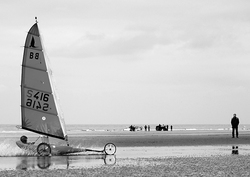
\includegraphics{zeilwagen}
  \end{center}
\end{oefening}

\begin{oefening}
  Beschouw de baan van een kogel die loodrecht de lucht in wordt geschoten met een beginsnelheid van $25\mpers$. De baan van de kogel wordt beschreven door de vergelijking
  $$y=25t-\frac{1}{2}gt^2\;.$$
  Hierbij is $t$ de tijd (in seconden), $y$ is de hoogte (in meter) en $g=9.81\mpers^2$ is de valversnelling. De hoofdvraag is: {\em Wat is de snelheid van die kogel na 1 seconde?}

  Om dit op te lossen los je volgende deelvragen op:
  \begin{enumerate}[(a)]
  \item Bereken $\Delta t$ en $\Delta y$ in het interval $[1,3]$.
  \item Wat is nu de gemiddelde snelheid (in $\mpers$) van de kogel in dit tijdsinterval?
  \item Bereken de gemiddelde snelheid van de kogel in het tijdsinterval $[1,t]$, waarbij we $t$ steeds dichter laten naderen tot $1$. Hiervoor maak je best een tabel met twee kolommen. In de linker kolom schrijf je de intervallen die steeds kleiner worden, begin met $[1,3]$, dan $[1,2]$, dan $[1,1.5]$, \ldots In de rechter kolom noteer je dan de berekening van de gemiddelde snelheid in dat interval.
  \item Naar welk getal nadert de gemiddelde snelheid?
  \end{enumerate}
\end{oefening}

\begin{oefening}
  Bij een wielrenner in een tijdrit worden op bepaalde plaatsen tussentijden genoteerd. Die vind je in de volgende tabel:

  \begin{center}
    \begin{tabular}{r|cccccccc}
      tijd $t$ (min) & 0 & 10 & 18 & 34 & 44 & 60 & 78 & 94\\
      \hline
      afstand $s$ (km) & 0 & 8 & 12 & 18 & 23 & 29 & 37 & 45\\
    \end{tabular}
  \end{center}

  \begin{enumerate}[(a)]
  \item Bereken het differentiequotiënt op het tijdsinterval $[0,10]$.
  \item Welke betekenis heeft dit getal voor de wielrenner? (Omcirkelen wat juist is.)
    \begin{enumerate}[(A)]
    \item Het is de afgelegde afstand in die periode.
    \item Het is de snelheid gedurende die periode.
    \item Het is de gemiddelde snelheid gedurende die periode.
    \item Het is de verlopen tijd in die periode.
    \end{enumerate}
  \item Je maakt bij deze tabel een grafiek door de punten met lijnstukken te verbinden. Op de horizontal as komt de tijd $t$ in minuten, op de verticale as de afgelegde afstand $s$ in kilometer. Bereken de rico van het lijnstuk dat hoort bij het interval $[44,60]$.
  \item Bereken voor het tijdsinterval $[18,44]$ de waarde $\dfrac{\Delta s}{\Delta t}$ in twee decimalen nauwkeurig.
  \item Welke betekenis hebben de bij (c) en (d) gevonden getallen voor de grafiek? (Omcirkelen wat juist is.)
    \begin{enumerate}[(A)]
    \item Ze geven de helling weer van het lijnstuk door de punten op de grafiek bij het begin en het einde van het tijdsinterval.
    \item Ze geven de totale toename van de afstand weer op het tijdsinterval.
    \item Ze geven de gemiddelde toename van de afstand per minuut weer op het tijdsinterval.
    \end{enumerate}
    \begin{center}
      
\includegraphics{tijdrit}
    \end{center}
  \end{enumerate}

\end{oefening}

\newpage
\section{Toepassingen}

\begin{oefening}\\
\begin{minipage}{0.75\textwidth}
  Het verband tussen het aantal graden Fahrenheit ($F$) en het aantal graden Celsius ($C$) wordt gegeven door$$F=1.8C+32\;.$$
  Bij welke temperatuur $T$ is het zowel $T$ graden Celsius als $T$ graden Fahrenheit?
\end{minipage}
\begin{minipage}{0.2\textwidth}
  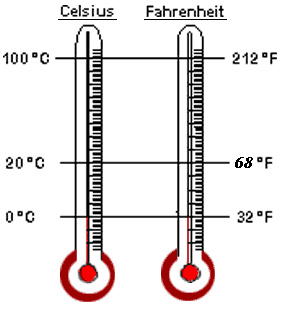
\includegraphics[width=\textwidth]{CelsiusFahrenheitThermo}
\end{minipage}
\end{oefening}

\begin{oefening}
  Na de bereiding van een ovenschotel op een temperatuur van $180\grC$ wordt de oven afgezet. Telkens wanneer er $5$ minuten voorbij zijn, is de temperatuur $10\grC$ gezakt.
  \begin{enumerate}[(a)]
  \item Bepaal de oventemperatuur een half uur na het uitzetten. (Tip: stel een functiewaardentabel op.)
  \item Met welke formule kun je de oventemperatuur $T$ berekenen op een willekeurig tijdstip $t$? (Maw. stel een functievoorschrift op.)
  \item Teken de grafiek. Houd er rekening mee dat, als de temperatuur tot $20\grC$ is gedaald, het afkoelingsproces stopt.
  \end{enumerate}
\end{oefening}

\begin{oefening}
  Je bent lid van een comité dat een spaghetti-avond organiseert ten voordele van je sportclub. Je doel is om voor 1500 euro spaghetti-tickets te verkopen. Hoeveel moet je vragen voor een ticket voor een volwassene en hoeveel voor een ticket voor een een kind, rekening houdend met de aanwezigheid van 200 volwassenen en 100 kinderen vorig jaar.

  Dit probleem heeft vele oplossingen. Je zou bijvoorbeeld 6 euro per volwassene en 3 euro per kind kunnen vragen of 4 euro per volwassene en 7 euro per kind of \ldots.
  \begin{enumerate}[(a)]
  \item Noteer een functievoorschrift voor dit probleem.
  \item Het comité beslist aan alle volwassenen $5.5$ euro te vragen. Hoeveel zal dan voor elk kind gevraagd worden?
  \end{enumerate}
\end{oefening}

\begin{oefening}
  Een vijver heeft de vorm van een cilinder. De diameter bedraagt $2$ meter en hij is $80$ cm met water gevuld. Door verdamping daalt het waterpeil dagelijks gemiddeld met $0.3$ cm. Na hoeveel dagen is de vijver leeg?
\end{oefening}

\begin{oefening}
  Je gooit een bal van het dak van de hoogste verdieping van een hoog gebouw ($60$ meter hoog). Je kunt de hoogte van de vallende bal weergeven door het voorschrift:
  $$h=60-\frac{1}{2}gt^2$$
  waarbij:
  \begin{itemize}
  \item $h$ de hoogte uitgedrukt in meters is,
  \item $g=9.81 \;m/s^2$ de valversnelling is,
  \item $t$ het tijdstip uitgedrukt in seconden is.
  \end{itemize}
  \begin{enumerate}[(a)]
  \item Maak een tabel en een grafiek van de val.
  \item Na hoeveel seconden bereikt de bal de grond (rond af op een honderdste van een seconde)?
  \end{enumerate}
\end{oefening}

\begin{oefening}

  \begin{minipage}{0.7\textwidth}
    In 1971 demonstreerde astronaut David Scott dat op de maan een veer en een hamer even snel vallen, omdat er op de maan geen atmosfeer en dus geen luchtweerstand is. Op de maan is de valversnelling $g=1.65 \mpers^2$.\\

    \begin{enumerate}[(a)]
    \item Je laat op de maan een hamer en een veer vallen vanaf $5$ meter. Na hoeveel seconden bereiken ze de maanbodem (rond opnieuw af tot op een honderdste van een seconde)?
    \item Wanneer bereikt de hamer de aardbodem bij dezelfde proef?
    \end{enumerate}
  \end{minipage}
  \begin{minipage}{0.29\textwidth}
    \vspace*{-0.4cm}
    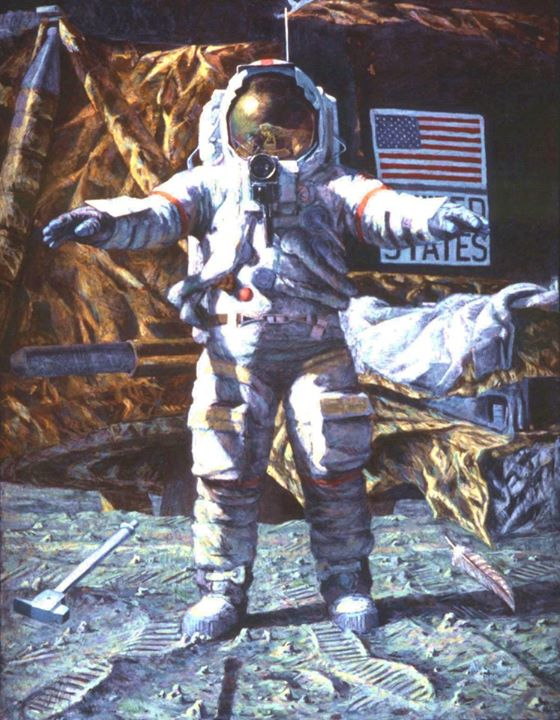
\includegraphics[width=1\textwidth]{hammerfeather}
  \end{minipage}

\end{oefening}

\begin{oefening}
  Is het mogelijk dat een rechthoek een omtrek heeft van $52 \cm$ en een oppervlakte van $148.75\cm^2$? Verklaar.
\end{oefening}


\begin{oefening}
  Twee schepen verlaten tegelijkertijd de haven van Zeebrugge. Het schip 'De Regenboog' vaart naar het westen en het schip 'De Viking' vaart naar het noorden. Na verloop van tijd bevinden ze zich op $270$ km afstand van elkaar. 'De Viking' heeft $50 \km$ meer gevaren dan 'De Regenboog'.
  \begin{enumerate}[(a)]
  \item Maak een schets van de situatie.
  \item Bereken van elk schip de afgelegde afstand tot de haven van Zeebrugge (rond af op $1 \km$).
  \end{enumerate}
  \begin{center}
    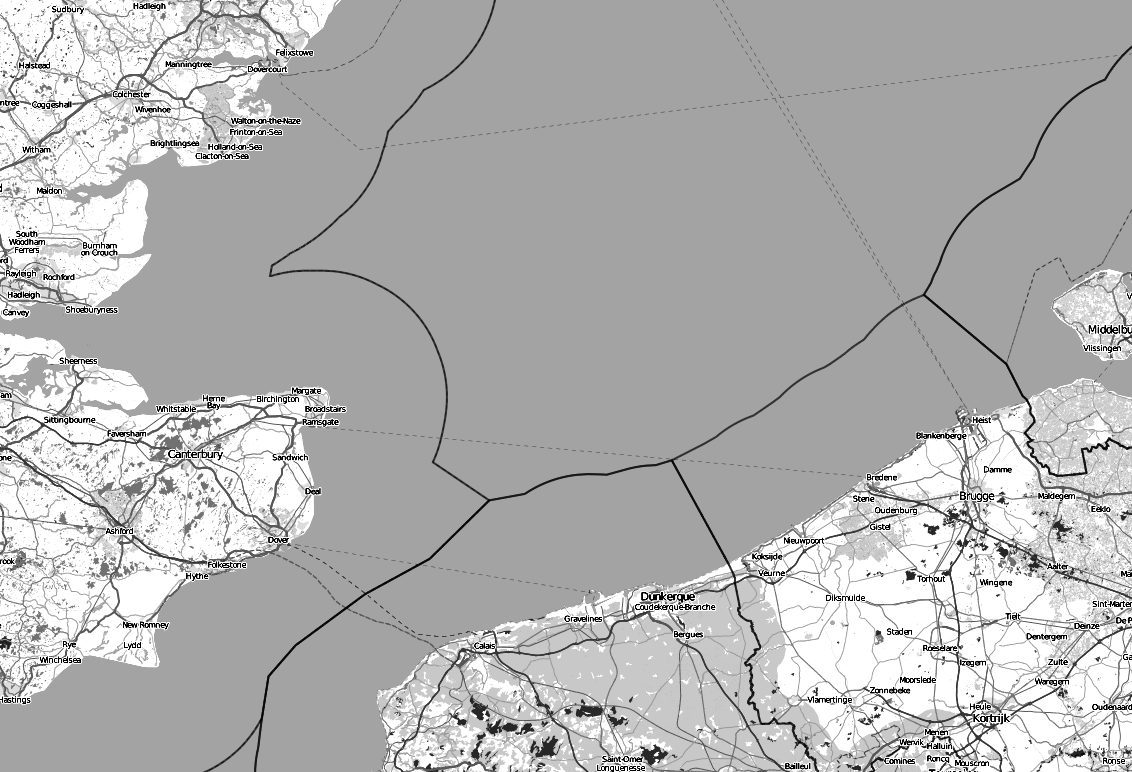
\includegraphics[width=\textwidth]{zeebrugge}
  \end{center}
\end{oefening}

\pagebreak

\section*{Het raadsel van Diophantus}

\subsection*{Diophantus}

Uit wikipedia:



\begin{wrapfigure}[16]{r}{0.4\textwidth}
  \vspace{-2cm}
  
\includegraphics[width=0.4\textwidth]{diophantus}
\end{wrapfigure}

\singlespacing

Diophantus van Alexandrië was een Griekse wiskundige, afkomstig uit Alexandrië. Wanneer hij leefde is niet erg duidelijk, het moet ergens tussen de 1e eeuw v.Chr. en de 4e eeuw na Chr. geweest zijn. Als meest waarschijnlijke datum geldt het midden van de 3e eeuw. Hij zou 84 jaar oud geworden zijn.

Binnen de Griekse wiskunde neemt Diophantus een bijzondere positie in. Waar de andere Griekse wiskundigen zich voornamelijk met de meetkunde bezighielden, en de andere aspecten van de wiskunde vanuit de meetkunde beschouwden, hield Diophantus zich bezig met algebra als een 'doel op zich'.

Hij ontwierp hiervoor een van de eerste schrijfsystemen voor algebraïsche vergelijkingen. Zijn methode kon vergelijkingen aangeven met alle machten van de onbekende van -6 tot 6, maar had als nadeel dat het niet met meerdere onbekenden kon werken. Ook was hij mogelijk de eerste die negatieve getallen in zijn berekeningen gebruikte, hoewel hij ze niet accepteerde als oplossingen voor vergelijkingen.

Zijn werk houdt zich bezig met datgene wat tegenwoordig naar hem als Diophantische vergelijkingen bekendstaan: polynomen met rationale coëfficiënten, waarvoor rationale oplossingen gezocht worden. Diophantus is er wel voor bekritiseerd dat hij slechts enkelvoudige oplossingen geeft, ook als een probleem oneindig veel oplossingen heeft, maar dat bezwaar is maar zeer gedeeltelijk terecht: in zijn methodes worden willekeurige getallen toegevoegd, en door deze te variëren krijgt men ook de andere mogelijkheden.

Diophantus schreef zijn werk op in de Arithmetika. Dit bestond uit 13 delen, waarvan echter lange tijd slechts 6 delen (1-3 en 8-10) bekend waren. Pas in 1982 werden 4 verdere delen (4-7) teruggevonden, zij het in Arabische vertaling. De laatste 3 delen zijn verdwenen. Het was in de kantlijn van Diophantus' Arithmetika dat Fermat zijn beroemde 'laatste' stelling schreef.

\subsection*{Raadsel}

Bepaal hoe oud Diophantus werd aan de hand van het volgende raadsel:

{\em God vergunde hem een zesde deel van zijn leven een jongen te zijn. Na een twaalfde deel kreeg hij een bebaard gelaat. Na nog eens een zevende deel ontstak hij het huwelijksvuur. Vijf jaar na zijn huwelijk kreeg hij een zoon, een geliefd maar ongelukkig kind. Na het bereiken van de helft van zijn vaders volle levensjaren sloeg het wrede noodlot toe. De vader had de laatste vier jaar van zijn leven om over het verdriet heen te komen. }

\section*{Peilingen naar vroeger}

\begin{oefening}
  $(2c-5)^2=$
  \begin{center}
    \begin{enumerate}[(A)]
    \itemsep.5em
    \item $4c^2+25$
    \item $4c^2-25$
    \item $4c^2-10c+25$
    \item $4c^2-20c+25$
    \end{enumerate}
  \end{center}
\end{oefening}

\begin{oefening}
  Hoe breed mag een rechthoekig glazen blad met een lengte van $3.35$ meter maximaal zijn om door een deuropening van $2.15$ meter hoog en $0.85$ meter breed te kunnen? Rond af op 0.01 meter. Je hoeft geen rekening te houden met de dikte van het glas.
\end{oefening}

\begin{oefening}
  Bereken en vereenvoudig: $$3\sqrt{32}-\sqrt{8}$$
\end{oefening}

\begin{oefening}
  Bereken en vereenvoudig:
  $$-2a-\left(\left(3b+2a\right)-3\left(a+b\right)\right)$$
\end{oefening}

\begin{oefening}
  Bepaal van de functie $f$, waarvan hieronder de grafiek werd getekend, alle nulwaarden en alle extrema.

  \begin{center}
    \definecolor{cqcqcq}{rgb}{0.7529411764705882,0.7529411764705882,0.7529411764705882}
    \begin{tikzpicture}[line cap=round,line join=round,>=triangle 45,x=3.0cm,y=3.0cm]
      \draw [color=cqcqcq,, xstep=0.5cm,ystep=0.5cm] (-1.2260478713808156,-1.191325606264551) grid (2.1500561653109176,1.1333223003558153);
      \draw[->,color=black] (-1.2260478713808156,0.) -- (2.1500561653109176,0.);
      \foreach \x in {-1.,-0.5,0.5,1.,1.5,2.}
      \draw[shift={(\x,0)},color=black] (0pt,2pt) -- (0pt,-2pt) node[below] {\footnotesize $\x$};
      \draw[->,color=black] (0.,-1.191325606264551) -- (0.,1.1333223003558153);
      \foreach \y in {-1.,-0.5,0.5,1.}
      \draw[shift={(0,\y)},color=black] (2pt,0pt) -- (-2pt,0pt) node[left] {\footnotesize $\y$};
      \draw[color=black] (0pt,-10pt) node[right] {\footnotesize $0$};
      \clip(-1.2260478713808156,-1.191325606264551) rectangle (2.1500561653109176,1.1333223003558153);
      \draw[line width=2.pt,smooth,samples=100,domain=-1.2260478713808156:2.1500561653109176] plot(\x,{1.0/2.0*sin((2.0*3.1415926535*(\x))*180/pi)});
      \draw (1.2,0.7) node[anchor=north west] {$f$};
      \begin{scriptsize}
        \draw[color=black] (-1.7195885038632934,0.4538098353437082) node {$f$};
      \end{scriptsize}
    \end{tikzpicture}
  \end{center}
\end{oefening}

\end{document}
